\textit{Cette phase d'analyse est un élément indispensable à la bonne réalisation du projet. }

\section{ORM}
\subsection{Qu'est-ce qu'un ORM ?}
\subsection{Pourquoi ?}

\section{Le modèle}
\subsection{Modèle réellement rencontré}
\begin{figure}[H]
\centering
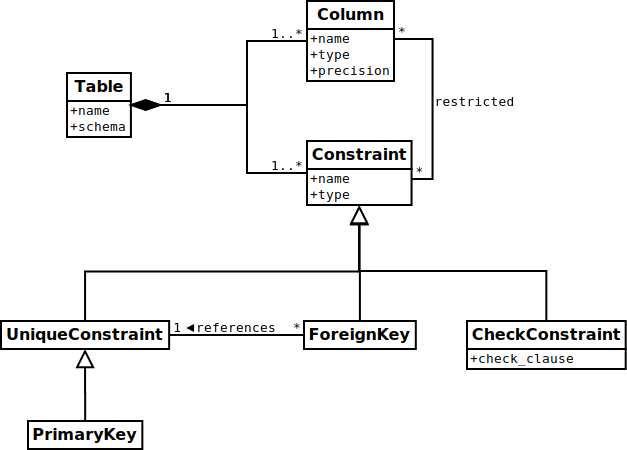
\includegraphics[width=\textwidth]{files/diag_class_ameliore}
\caption{Diagramme de classe réellement rencontré.}
\label{figure:diag_classe_reel}
\end{figure}
	\subsection{Attributs}
		Gestion des types génériques
	\subsection{Tables}
	\subsection{Contraintes}

\section{Compatibilité avec les SGBD}

\section{Générateur de graphes}
  \subsection{différentes librairies}
		\begin{itemize}
			\item jung
				entrée : un fichier dot\\
				inconvénients : dernières fonctionnalités dot non prise en charqe.
			\item grappa
				 entrée : fichier dot
			\item graphviz
		\end{itemize}	
  \subsection{Notre choix}
		\verb+//Notre choix c'est porté sur la commande DOT fournit par GraphViz+


\section{L'IHM}	
	\subsection{les choix possibles}
			\subsubsection{GUI : \og Graphical User Interface \fg{}}
			\subsubsection{CLI : \og Command Line Interface \fg{}}
				philosophie KISS « Keep it simple, Stupid! »
